\documentclass[twocolumn]{article}
\usepackage{color}
\usepackage{cite}
\usepackage{draftwatermark}
\usepackage{multirow}
\usepackage{listings}
\usepackage{float}
\usepackage{amsfonts}
\usepackage{amssymb}
\usepackage{amsmath}
\usepackage{amsthm}
\usepackage{epsfig}
\usepackage{epstopdf}
\usepackage{titling}
\usepackage{url}
\usepackage{enumitem}
\usepackage{array}
\usepackage[utf8]{inputenc}
\usepackage[english]{babel}
\usepackage{tikz}
\usepackage{algorithm}
\usepackage[noend]{algpseudocode}
\usepackage{abstract}

\newtheorem{definition}{Definition}
\newtheorem{constraint}{Constraint}
\newtheorem{assumption}{Assumption}
\newtheorem{proposition}{Proposition}

\date{Created: February 8, 2023\\Source: RingsNetwork/whitepaper repository\\Timestamp: 2023-02-08T13:27:55Z\\Last updated: July 4, 2026}
\usetikzlibrary{shapes,arrows,positioning,patterns,through}
\SetWatermarkText{Preview}
\SetWatermarkScale{1}
\setlength\parskip{.5\baselineskip}

\definecolor{pagecolor}{rgb}{1,0.98,0.9}
\pagecolor{pagecolor}

\tikzset{
  dot node/.style={
    shape=circle,
    fill=white,
    draw,
    inner sep=+0pt,
    minimum size=+5mm
  },
  dotdot node/.style 2 args={
    dot node,
    label={[shape=circle,fill=black,outer sep=+0pt,inner sep=+0pt,minimum size=+3mm,name=ddd-#1,#2]center:}
  },
  arc style/.style={
    |<->|,
    shorten >=+-.5\pgflinewidth,
    shorten <=+-.5\pgflinewidth,
  }
}

\author{
  Ryan J. Kung \\ ryankung@ieee.org \\
}
\title{Rings: A peer-to-peer network for the sovereign age}

\begin{document}
\twocolumn[
  \begin{@twocolumnfalse}
    \maketitle
    \begin{abstract}

      Rings Network is a decentralized peer-to-peer network for the sovereign age. This paper specifies a target architecture in which browsers and native devices participate as first-class nodes, identities are addressed as DIDs on a Chord overlay, resources and services are mapped into the same identifier space, and applications compose privacy-preserving protocols such as encrypted messaging, offline mailboxes, hidden service descriptors, ranking, and sidecar ordering. The formal core models namespaces as objects in the slice category $\mathbf{Set}/R$ for $R=\mathbb{Z}/2^{160}\mathbb{Z}$, places them by post-composition with the live Chord owner map, and composes effectful protocol transitions as writer-monad Kleisli morphisms. The ideal model also updates directions that have been superseded: Chord identifiers are treated as an additive circular space for routing and placement, cryptographic groups and fields are separate protocol carriers, and message relay, ranking, and sequencing are specified as Rings protocols rather than inherited wholesale from unrelated systems.

  ~\\
  ~\\
\end{abstract}
\end{@twocolumnfalse}
]
\section{Introduction and Motivation}

Centralized systems have long posed privacy, security, and data-control risks to Internet users \cite{Kshetri2014, Kokkonen2018, G2016, tim}. Rings studies a narrower design problem: how can browser and native runtimes share one peer-to-peer overlay without treating identity, routing, storage, and application protocols as centralized services?

This paper makes four contributions:
\begin{itemize}[itemsep=2pt,topsep=0pt,parsep=0pt]
\item it models Rings identifiers as an additive circular carrier used for Chord placement, not as a cryptographic field;
\item it adopts Correct Chord as the maintenance reference before adding Rings-specific DID, VID, storage, mailbox, and service semantics;
\item it defines namespace placement categorically and protocol execution through a writer-monad effect boundary;
\item it states the verification boundary for lookup, storage placement, and protocol effects without claiming full asynchronous liveness or Byzantine fault tolerance.
\end{itemize}

\subsection{Browser Native}

The Rings Network is characterized as a browser-native network at the protocol level: a browser tab can own an identity, establish peer-to-peer transport, participate in routing, store replicated state within its capability profile, and host applications without depending on an application server. Native and browser environments expose different operating-system capabilities, but the ideal model gives both the same overlay authority and isolates environment-specific IO behind adapters.


The browser communication layer uses WebRTC \cite{webrtc-standard} and WebAssembly \cite{webassembly}. WebRTC provides browser-to-browser data channels after peers exchange connectivity information. WebAssembly lets the same protocol core run inside browser capability boundaries while native nodes use host adapters.

Moreover, the integration of WebRTC and WebAssembly allows decentralized applications to run on top of the same overlay. The target application space includes secure file sharing, decentralized web publishing, private mailboxes, verifiable computation, relay/tunnel services, and market or exchange protocols that can be expressed as namespace-scoped applications.

\subsection{Proof Based DID}


Decentralized Identifiers (DIDs) in Rings are protocol identities located on the Chord identifier circle. A participant proves control of a DID through an account proof and a delegated session proof. Rings does not require a W3C DID-document resolver in the core overlay path; DID resolution is a routing and proof problem inside the overlay.

The target DID proof system is pluggable but not arbitrary. Each proof family specifies a verifier, a domain-separated transcript, DID derivation, signature encoding, replay bounds, and whether the public key is recoverable from the signature or carried explicitly. This keeps Rings compatible with multiple cryptographic ecosystems without losing a uniform proof boundary.

The DID proof boundary is therefore an authorization interface: routing locates an identifier, while protocol verification decides whether a signed operation is valid for that identifier.


\subsection{Lookup Protocol and Encryption}

The Rings Network leverages the Chord algorithm\cite{Chord} for overlay lookup. The network is organized as a circular identifier space, and each node maintains successor, predecessor, and finger-table state to route messages and storage operations toward a destination DID or resource identifier.

In conjunction with the lookup protocol, the Rings Network uses signed message payloads and end-to-end encryption. Peers exchange signed public-key handshakes, then carry ordered ciphertext frames inside signed message envelopes. Secret sharing, private storage, and verifiable computation use their own cryptographic fields or groups; the Chord identifier space itself is not a finite field.

Lookup and encryption have distinct security roles. Chord routes to a DID or VID owner under the overlay assumptions; signed sessions and end-to-end encryption protect message authenticity and payload confidentiality.

\subsection{Data and Service Provision}

Rings maps resources and service records into the same 160-bit identifier space used by the Chord overlay. Virtual DIDs represent data, mailboxes, service descriptors, subrings, and application-specific rendezvous points. A virtual DID has no account proof of its own; its authenticity comes from signed entry operations, encrypted payloads, capability descriptors, and the application protocol that defines how the resource may be read or updated.

\section{Related Work}
Several decentralized networks, including Tor, GnuNet, Nym, and IPFS, address privacy, security, censorship resistance, or content routing. Rings differs by making browser-capable Chord placement the shared substrate for identity, storage, and protocol rendezvous.

Distributed Hash Tables (DHTs\cite{DHT}) are common in P2P systems. Networks such as Edonkey\cite{Edonkey}, Ethereum\cite{Ethereum}, IPFS\cite{IPFS}, and Libp2p\cite{Libp2p} use Kademlia-derived routing \cite{Kademlia}. Rings instead employs Chord for structured routing, which gives the model a circular order for successor, predecessor, and finger-table reasoning. Broadcast and gossip behavior is treated as Rings protocol behavior rather than inferred from the DHT alone.

Rings belongs to the structured P2P family. Unstructured overlays can be more tolerant of arbitrary churn and partial knowledge, while structured overlays provide deterministic lookup targets and compact routing state when their maintenance assumptions hold. Rings chooses the latter tradeoff because DID and VID placement need a stable owner relation.

In terms of P2P communication protocols, the Chord protocol is employed by Rings Network, whereas IPFS and Ethereum utilize Kademlia-derived systems. Rings' design goal is to use the structured ring as the base for lookup, relay, storage placement, and service rendezvous, while keeping privacy-sensitive network addresses out of application-level identifiers whenever possible.

In contrast, Tor network and Nym network are not structured P2P networks but rather relay networks that are decentralized but not P2P. Rings takes a different path by making the structured overlay itself the routing and service-discovery substrate. This reduces dependence on fixed relay infrastructure, while traffic-analysis and metadata-resistance claims still depend on the selected relay, ranking, mailbox, and cover-traffic protocols.

Finally, Rings treats browser runtimes as first-class peers. Browser, mobile, and native nodes differ in persistence and transport capabilities, but the target protocol gives them the same identity and overlay authority when they satisfy the same proof and session rules.
\section{The Rings Network Architecture}
The Rings Network architecture is not a direct restatement of the TCP/IP reference model \cite{TCP_IP}. It is a sovereign-network architecture organized around six cooperating layers: identity, transport, overlay, extension runtime, protocol, and application.

\begin{itemize}[itemsep=2pt,topsep=0pt,parsep=0pt]
\item Identity Layer: DID addressing, account proofs, delegated sessions, and virtual-resource identities.
\item Transport Layer: browser and native peer-to-peer data channels, NAT traversal, and transport capability profiles.
\item Overlay Layer: the Chord DHT maintains successor, predecessor, finger-table, storage, and message-routing state.
\item Extension Runtime Layer: namespace-scoped protocols are modeled as state transitions whose effects are interpreted by constrained shells.
\item Protocol Layer: relay, mailbox, ranking, sidecar sequencing, service discovery, private storage, and verifiable-computation protocols.
\item Application Layer: decentralized web, secure messaging, hidden services, proof applications, and user-defined sovereign applications.
\end{itemize}

\begin{figure}[htbp]
\centering
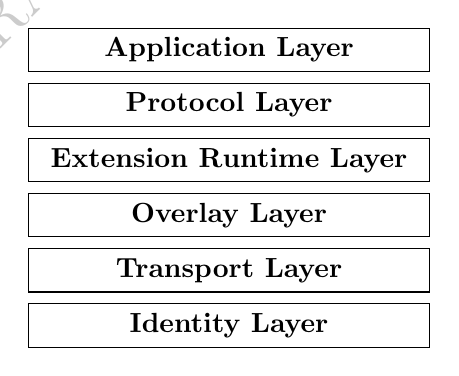
\begin{tikzpicture}[every node/.style={draw,minimum width=5.1cm,minimum height=.55cm,align=center,font=\bfseries}]
\node (1) at (4.5,0) {Identity Layer};
\node (2) at (4.5,0.7) {Transport Layer};
\node (3) at (4.5,1.4) {Overlay Layer};
\node (4) at (4.5,2.1) {Extension Runtime Layer};
\node (5) at (4.5,2.8) {Protocol Layer};
\node (6) at (4.5,3.5) {Application Layer};

\end{tikzpicture}
\caption{Layers of Rings Network}
\end{figure}





\subsection{Identity Layer}

The design goal of Rings Network is to make the same overlay and identity model available from multiple runtime surfaces. Native nodes, mobile nodes, embedded nodes, and browser nodes share DID addressing, delegated sessions, Chord routing, and message semantics. Each runtime supplies the IO adapters available in that environment, so equality means equal protocol authority rather than identical local resources.

The identity layer owns DID derivation, account-proof verification, delegated sessions, and virtual-resource identities. It names who or what is allowed to sign a protocol operation; it does not decide transport reachability, overlay placement, or application-specific authorization policy.

\subsection{Transport Layer}
The transport layer uses WebRTC data channels and native transport adapters to give browser and non-browser nodes peer-to-peer connectivity. Browser nodes use the standardized SDP/ICE exchange to establish data channels; native adapters expose equivalent transport capabilities where a browser tab cannot.

Figure \ref{webrtc-standard-sdp} sketches the ordinary SDP/ICE exchange between two WebRTC peers:

 \begin{itemize}[itemsep=2pt,topsep=0pt,parsep=0pt]
  \item Node A gathers a list of ICE candidates and generates an SDP offer. The SDP offer includes information about the media streams and network addresses that Node A is willing to receive or transmit.
  \item Node A sends the SDP offer to Node B.
  \item Node B receives the SDP offer and starts gathering its own list of ICE candidates.
  \item Node B generates an SDP answer in response to the SDP offer received from Node A. The SDP answer includes information about the media streams and network addresses that Node B is willing to receive or transmit.
  \item Node B sends the SDP answer and its list of ICE candidates back to Node A.
  \item Node A receives the SDP answer and the list of ICE candidates from Node B.
  \item Node A and Node B use the ICE candidates and SDP information to establish a connection and establish a peer-to-peer communication channel.
  \end{itemize}

\begin{figure}[htbp]
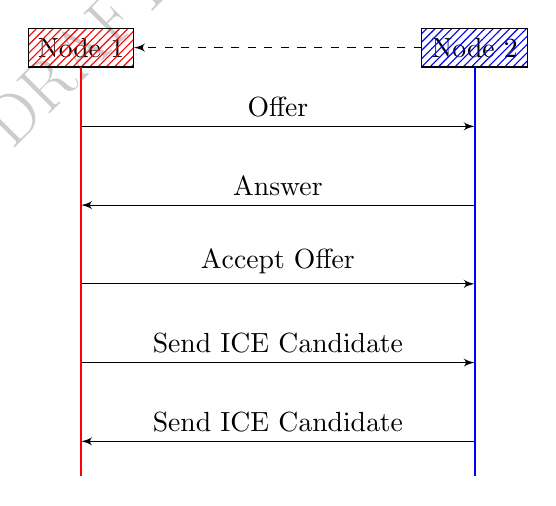
\begin{tikzpicture}[node distance=5cm,auto,>=latex']
  \node (A) {Node 1};
  \node (B) [right of=A] {Node 2};
  \draw[->] (A |-, -1) -- node[above] {Offer} (B |-, -1);
  \draw[->] (B |-, -2) -- node[above] {Answer} (A|-, -2 );
  \draw[->] (A |-, -3) -- node[above] {Accept Offer} (B |-, -3);
  \draw[->] (A |-, -4) -- node[above] {Send ICE Candidate} (B |-, -4);
  \draw[->] (B |-, -5) -- node[above] {Send ICE Candidate} (A |-, -5);
  \draw[->,dashed] (B) -- (A);
  \draw[pattern=north east lines, pattern color=red] (A.south west) -- (A.south east) -- (A.north east) -- (A.north west) -- cycle;
  \draw[pattern=north east lines, pattern color=blue] (B.south west) -- (B.south east) -- (B.north east) -- (B.north west) -- cycle;
  \draw[red, thick] (A.south) -- ++(0,-5.2cm);
  \draw[blue, thick] (B.south) -- ++(0,-5.2cm);
\end{tikzpicture}

\caption{Standard SDP/ICE exchange}
\label{webrtc-standard-sdp}
\end{figure}

Rings compresses the overlay handshake by carrying the offer and locally gathered ICE candidates in one request, and the answer and responder candidates in one response. Figure \ref{webrtc-rings-sdp} shows the single round-trip form. The optimization changes the Rings signaling protocol, not the WebRTC security model itself.


\begin{figure}[htbp]
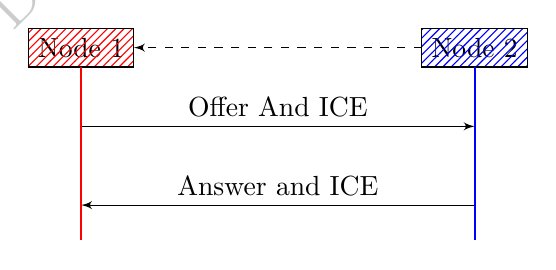
\begin{tikzpicture}[node distance=5cm,auto,>=latex']
  \node (A) {Node 1};
  \node (B) [right of=A] {Node 2};
  \draw[->] (A |-, -1) -- node[above] {Offer And ICE} (B |-, -1);
  \draw[->] (B |-, -2) -- node[above] {Answer and ICE} (A|-, -2 );
  \draw[->,dashed] (B) -- (A);
  \draw[pattern=north east lines, pattern color=red] (A.south west) -- (A.south east) -- (A.north east) -- (A.north west) -- cycle;
  \draw[pattern=north east lines, pattern color=blue] (B.south west) -- (B.south east) -- (B.north east) -- (B.north west) -- cycle;
  \draw[red, thick] (A.south) -- ++(0,-2.2cm);
  \draw[blue, thick] (B.south) -- ++(0,-2.2cm);
\end{tikzpicture}

\caption{Rings single round-trip SDP/ICE exchange}
\label{webrtc-rings-sdp}
\end{figure}

\subsection{Overlay Layer}

The Rings Network is a structured peer-to-peer network that incorporates a distributed hash table (DHT) to facilitate efficient and scalable lookups. The Chord algorithm is utilized to implement lookup within the DHT, thereby enabling message routing and replicated storage operations in a peer-to-peer setting. Availability depends on transport connectivity, stabilization progress, redundancy settings, and churn; the DHT gives the protocol a structured basis for routing rather than a standalone availability guarantee.

Each node in the Rings Network occupies a point in an $m$-bit identifier space with $2^m$ possible identifiers. The live node set is a finite subset of that space. A key is owned by the first live node encountered clockwise from the key. Each node stores predecessor and bounded successor-list state as its safety root, and may also store finger entries as routing hints.

To maintain the robustness of the network in the event of node failures or departures, each node records a segment of the ring adjacent to it, including the preceding and following nodes. The predecessor and successor list are maintained by join, rectify, and stabilize operations; finger tables are repaired separately and are not the authoritative source for immediate neighbor correctness.

The Rings Network uses Chord-style finger routing to reduce query times and improve lookup efficiency. When a node seeks to look up a key, it forwards the query to the closest known predecessor or successor of the key, as determined by the information stored in its finger table and successor list, until the responsible node is found. This approach reduces the number of nodes that must be traversed to locate the responsible node, providing a scalable solution for data storage and retrieval within a peer-to-peer network.

In this way, the Chord algorithm provides a scalable way to store and retrieve data in a peer-to-peer network. The use of the hash function and finger table allows efficient routing of queries and updates, while redundancy, stabilization, and repair policies provide the basis for availability and robustness against node failures.

\begin{figure}[h]
    \begin{center}

  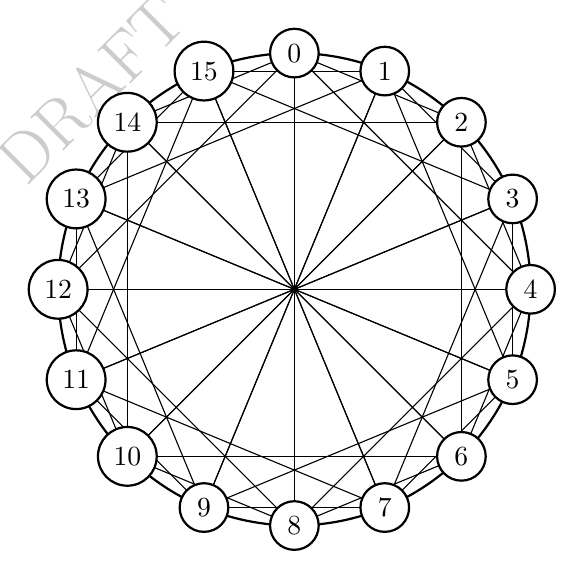
\begin{tikzpicture}[node distance=5cm,auto,>=latex']
    \xdef\N{16}
    \xdef\S{3}
    \xdef\deltadegree{360/\N}
    \draw[thick] (0,0) circle (\S);

    \foreach \i in {0,...,15} {
        % % predecessor
        % \pgfmathsetmacro{\result}{mod(\i-1,\N)}
        % \draw[color=red] (-\i*\deltadegree+90:\S) -- (-1*\result*\deltadegree+90:\S);

        % % successor
        % \pgfmathsetmacro{\result}{mod(\i+1,\N)}
        %     \draw (-\i*\deltadegree+90:\S) -- (-1*\result*\deltadegree+90:\S);

      % fingers
      \foreach \j in {1,...,4}{
            \pgfmathsetmacro{\result}{mod(\i+2^\j,\N)}
            \draw (-\i*\deltadegree+90:\S) -- (-1*\result*\deltadegree+90:\S);
        }
    }
    \foreach \i in {0,...,15}
    \node (\i) [circle,fill=white,draw=black,thick] at (-\i*\deltadegree+90:\S) {\i};
  \end{tikzpicture}
    \end{center}
      \caption{Chord algorithm, lookup protocol}
    \label{dht}

    \end{figure}
In the DHT, as illustrated in Figure \ref{dht}, all nodes have the capability to perceive their own predecessor and successor through the join and stabilization algorithms. The predecessor of a node is determined as the node with the largest identifier that precedes the identifier of the current node in the identifier space. Conversely, the successor of a node is defined as the node with the smallest identifier that follows the identifier of the current node in the identifier space. These two nodes, the predecessor and the successor, are considered the immediate neighbor nodes of a particular node within the network.

\subsection{Extension Runtime Layer}

The extension runtime layer is the interpreter boundary for namespace-scoped protocol logic. Protocol handlers are modeled as pure state transitions that return effect descriptions, while the runtime supplies capability-limited host calls for storage, transport, timers, and cryptographic verification. This keeps extension behavior replayable and testable without giving each extension direct ambient access to the node process.

WebAssembly (Wasm) is the browser-side module format used by this boundary \cite{webassembly}. In Rings, Wasm is relevant because it lets protocol code run behind browser capability checks while native nodes expose equivalent adapters.

\begin{figure}[htbp]
  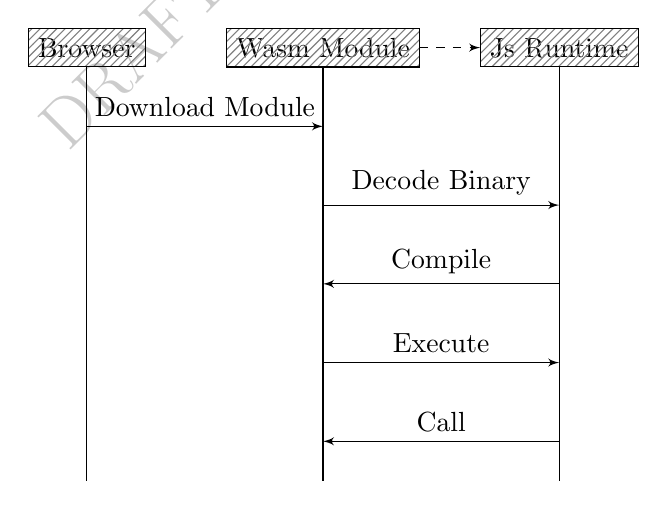
\begin{tikzpicture}[node distance=3cm,auto,>=latex']
  \node (A) {Browser};
  \node (B) [right of=A] {Wasm Module};
  \node (C) [right of=B] {Js Runtime};
  \draw (A) -- (A |-, -5.5);
  \draw (B) -- (B |-, -5.5);
  \draw (C) -- (C |-, -5.5);
  \draw[->] (A |-, -1) -- node[midway, above] {Download Module} (B |-, -1);
  \draw[->] (B |-, -2) -- node[midway, above] {Decode Binary} (C |-, -2);
  \draw[->] (C|-, -3) -- node[midway, above] {Compile} (B|-, -3);
  \draw[->] (B|-,-4) -- node[midway, above] {Execute} (C|-, -4);
  \draw[->] (C|-,-5) -- node[midway, above] {Call} (B|-,-5);
  \draw[pattern=north east lines, pattern color=gray] (A.south west) -- (A.south east) -- (A.north east) -- (A.north west) -- cycle;
  \draw[pattern=north east lines, pattern color=gray] (B.south west) -- (B.south east) -- (B.north east) -- (B.north west) -- cycle;
  \draw[pattern=north east lines, pattern color=gray] (C.south west) -- (C.south east) -- (C.north east) -- (C.north west) -- cycle;
  \draw[->,dashed] (B) -- (C);
\end{tikzpicture}
\caption{Wasm module execution boundary}
\end{figure}

The Rings Network provides multiple options for interacting with WebAssembly (Wasm) modules:

\begin{itemize}[itemsep=2pt,topsep=0pt,parsep=0pt]
\item Build browser applications using wasm-based frameworks such as Yew and Trunk.
\item Load the exported JavaScript/Wasm module directly from web applications.
\item Use a browser provider or extension workflow, where applications interact with a Rings provider surface and register namespace-scoped handlers.
\end{itemize}

\subsection{Protocol Layer}

In the protocol layer, the central design concept revolves around the utilization of a Decentralized Identifier (DID). A DID is a 160-bit Chord identifier in a space with $2^{160}$ points, represented as an element of the additive cyclic group $\mathbb{Z}/2^{160}\mathbb{Z}$. Addition, subtraction, and negation model clockwise offsets, biased ordering, finger targets, and affine replica placement. DID multiplication is outside the Rings routing model: cryptographic multiplication belongs to the fields or groups used by specific cryptographic protocols, not to Chord identifiers themselves.

However, elements in a circular identifier space cannot be compared by a single global less-than relation that is meaningful for every observer. For a fixed point $C$, Rings uses the biased order
\[
  A \leq_C B
  \quad\Longleftrightarrow\quad
  \delta_C(A) \leq \delta_C(B).
\]
This is the pullback of the ordinary order on $[0,M)$ along $\delta_C$. It is total for each fixed $C$, but changing $C$ changes the order; that observer-dependence is the reason Chord interval tests always name a reference point.


The DID, as an element of the Chord identifier space, also provides a placement target for resources and storage entries. Resource identifiers are derived into the same 160-bit space so the same lookup and placement logic can route storage, mailbox, service, and subring operations.


The DID architecture also encompasses signed Session and Message Relay modules. Sessions delegate a temporary session keypair from an account proof, and message payloads carry signed routing metadata so handlers can process system messages, storage messages, encrypted frames, mailbox operations, and namespace-scoped extension messages.

\subsection{Application Layer}

The nucleus of Rings Network is similar to the Actor Model\cite{Actor_Model}: inbound messages are decoded into typed protocol messages and handled by explicit handler traits. The extension runtime described above separates protocol logic into a pure state transition and an interpreter shell. This allows built-in and user-defined protocols to run behind namespace-scoped capabilities without adding a global command bus.

Rings exposes application-layer messages through Remote Procedure Calls (RPC) and Foreign Function Interface (FFI) surfaces. Rust and WebAssembly applications can call the protocol core directly, scripting environments can use RPC, and embedded runtimes can bind through FFI when their capability profile supports the required transport and storage adapters.

Additionally, applications can store data in the Distributed Hash Table (DHT), look up services, and register namespace-scoped protocols. In the ideal model, peer quality and global ranking provide admission and routing signals, while local counters remain the lowest-level evidence source.


\begin{figure}[htpb]
  \begin{center}
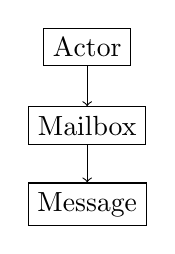
\begin{tikzpicture}
\node[rectangle, draw] (actor) {Actor};
\node[rectangle, draw, below of=actor] (mailbox) {Mailbox};
\node[rectangle, draw, below of=mailbox] (message) {Message};

\draw[->] (actor) -- (mailbox);
\draw[->] (mailbox) -- (message);
\end{tikzpicture}
\end{center}
\caption{Actor Model}

\end{figure}

Several application classes motivate Rings Network: decentralized chat, dWeb publishing, relay/tunnel services, browser proof applications, private mailbox delivery, and hidden-service style rendezvous. The model characterizes these applications by protocol class and requirement rather than by transient demo names.

\section{Algebraic Network}

\subsection{Classic Chord}

Rings builds on the Chord distributed hash table rather than inventing a new overlay from first principles. In Chord, nodes and keys are mapped by consistent hashing into an $m$-bit circular identifier space, usually written as $[0,2^m)$. The owner of a key is its successor: the first live node encountered when moving clockwise around the identifier circle. Each node stores at least its successor and predecessor, and it may maintain a finger table whose $i$-th entry points near $n + 2^i$ to accelerate lookup \cite{Chord}.

Chord lookup is a routing procedure over this circular order. If the target key lies between the local node and its successor, the successor is returned. Otherwise the query is forwarded to the closest preceding known node, usually obtained from the finger table, until a node can answer the successor relation. Periodic maintenance then repairs the local view: stabilization asks the current successor for topology information, notification lets a successor learn a better predecessor, and finger repair refreshes long-distance routing hints.

This base model gives Rings its first algebraic object: a circular identifier carrier with relative order, successor, predecessor, and finger relations. It also defines the separation between correctness and performance. The successor/predecessor structure is the safety-critical ring-maintenance state, while fingers optimize hop count without becoming the proof root for membership correctness.

\subsection{Correct Chord as Maintenance Model}

The original Chord paper is not enough as a formal maintenance model under churn. Zave's Correct Chord work shows that the original ring-maintenance protocol was not correct under its stated operating assumptions, then gives corrected operations, initialization constraints, and an inductive invariant for preserving reachability in Chord identifier spaces \cite{ZaveChordCorrect}. In particular, Correct Chord makes successor lists and a stable base of at least $r+1$ members central to the correctness argument, where $r$ is the successor-list length.

Rings adopts Correct Chord as the maintenance reference before adding Rings-specific semantics. The relevant transition family is join, rectify, and stabilize. Join introduces a node through a known peer and constructs a bounded successor list. Rectify processes a predecessor notification and accepts it only when it is a better predecessor candidate. Stabilize refines the successor list from the current successor's topology. Finger maintenance remains a routing optimization, and storage repair is a Rings extension layered on top of Chord placement.

\subsection{Rings as an Algebraic Object}

The Rings model is not merely "Chord plus applications." It is a family of protocol objects indexed over one circular carrier, with effects interpreted through a monadic runtime boundary. We use standard category-theoretic language for the placement construction \cite{MacLaneCategories}, and monadic language for effectful protocol composition \cite{MoggiMonads}.

\begin{assumption}[Overlay model]
The steady-state algebra below assumes a finite live set $N\subset R$, a successor-list length $r\geq 1$, and the Correct Chord stable-base condition $|N|\geq r+1$. Bootstrap rings with fewer nodes are initialization states, not instances of the steady-state lookup theorem. Nodes are fail-stop, not Byzantine, and modeled remote or repair actions are delivered under the fairness assumptions of the selected verification artifact.
\end{assumption}

\begin{definition}[Carrier and circular order]
Let
\[
  M = 2^{160},
  \qquad
  R = \mathbb{Z}/M\mathbb{Z}.
\]
For an observer $a \in R$, define clockwise distance and interval membership by
\[
  \delta_a(x) = (x-a) \bmod M,
\]
\[
  (a,b]_R =
  \{x \in R : 0 < \delta_a(x)
  \land \delta_a(x) \leq \delta_a(b)\}.
\]
The carrier operation used by the overlay is addition in $R$. Multiplication in $R$ is not a routing operation.
\end{definition}

For a nonempty finite live set $N \subset R$, the mathematical owner of a key $k$ is
\[
  \operatorname{owner}_N(k)
    = \arg\min_{n \in N} \delta_k(n).
\]
The predecessor and bounded successor sequence of node $n\in N$ are
\[
  \operatorname{pred}_N(n)
    = \arg\min_{p \in N\setminus\{n\}} \delta_p(n),
\]
\[
  \operatorname{Succ}^q_N(n)
    = \operatorname{take}_q
      \bigl(\operatorname{sort}_{\delta_n}(N \setminus \{n\})\bigr).
\]
The argmins are unique because $\delta_a$ is a bijection from $R$ to $\{0,\ldots,M-1\}$ for each fixed $a$. For a replication factor $r$, the intended storage set for key $k$ is
\[
  \operatorname{Rep}^r_N(k)
  =
  \{\operatorname{owner}_N(k)\}
  \cup\;
  \mathrm{set}\!\bigl(
    \operatorname{Succ}^{r-1}_N(\operatorname{owner}_N(k))
  \bigr).
\]
Correct Chord gives the maintenance discipline for making local successor-list state converge toward these mathematical functions; Rings adds typed identities, resources, storage, sessions, and extension protocols on top of them.

\begin{definition}[Rings object]
A Rings overlay state over $N$ is the tuple
\[
\mathcal{R}_N =
  (R,N,\operatorname{owner}_N,\operatorname{pred}_N,
   \operatorname{Succ}^r_N,\operatorname{Rep}^r_N,F,E)
\]
where $F$ is the sparse finger relation and $E$ is the replicated entry store indexed by VIDs. The safety root is $(\operatorname{pred},\operatorname{Succ}^r)$; $F$ is a performance witness, and $E$ is a protocol-indexed payload algebra.
\end{definition}

Rings' main categorical move is to put every routable thing in the slice category $\mathbf{Set}/R$. A DID namespace, a mailbox namespace, a service-descriptor namespace, and a subring namespace are all sets equipped with a derivation map into $R$:
\[
  H_\nu : X_\nu \longrightarrow R .
\]
DIDs are account-controlled elements of such a namespace. VIDs are resource-controlled or protocol-derived elements. Both are objects over the same carrier, not elements of the same cryptographic group.

For a fixed live topology $N$, the owner map induces a post-composition functor
\[
  \Omega_N:\mathbf{Set}/R \longrightarrow \mathbf{Set}/N.
\]
It maps an object $(X,H:X\to R)$ to $(X,\operatorname{owner}_N\circ H:X\to N)$ and maps a slice morphism $f$ to the same underlying function $f$. Thus namespace placement is the composite
\[
  P^N_\nu = \operatorname{owner}_N \circ H_\nu :
  X_\nu \longrightarrow N .
\]
\begin{proposition}[Placement functoriality]
If $f:X_\nu \to X_\mu$ is a morphism in $\mathbf{Set}/R$, then placement commutes with $f$:
\[
  H_\mu \circ f = H_\nu ,
\]
\[
  P^N_\mu \circ f = P^N_\nu .
\]
\end{proposition}
\begin{proof}
Post-compose the first equation with $\operatorname{owner}_N$. Identities and composition are preserved because $\Omega_N$ leaves the underlying function unchanged.
\end{proof}
This is the precise claim behind "DIDs, resources, mailboxes, service descriptors, and subrings share the same ring." They share placement by a commuting diagram over $R$; they do not share authorization, payload semantics, or cryptographic carrier laws.

\begin{constraint}[Carrier separation]
Overlay placement may use only
\[
  0,\quad +,\quad -,\quad \delta_a,\quad (a,b]_R,\quad
  \operatorname{owner}_N .
\]
Any protocol requiring multiplication, inversion, scalar multiplication, polynomial interpolation, pairings, or subgroup checks must name a separate carrier such as a finite field $\mathbb{F}_q$ or elliptic-curve group $\mathbb{G}$. The only bridge from bytes or proofs into $R$ is an explicit, domain-separated derivation map $H_\nu$.
\end{constraint}

\begin{proposition}[Rotation equivariance]
For every offset $t \in R$, define $T_t(x)=x+t$ and $N+t=\{n+t\mid n\in N\}$. Rings placement is independent of the absolute zero point:
\[
  \operatorname{owner}_{N+t}(k+t)
    = \operatorname{owner}_N(k)+t .
\]
Thus a diagram, storage policy, or test that depends only on circular offsets can be translated around the ring without changing its algebraic content.
\end{proposition}
\begin{proof}
For every $n\in N$, $\delta_{k+t}(n+t)=((n+t)-(k+t))\bmod M=\delta_k(n)$. Translation therefore preserves the ordering used by $\arg\min$, so the translated minimizer is the minimizer translated by $t$.
\end{proof}

\begin{definition}[Writer effect monad]
For an action alphabet $A$, let $A^*$ be the free monoid of finite action lists with identity $\epsilon$ and concatenation $\cdot$. The Rings effect monad is the writer monad over $A^*$:
\[
  \mathsf{T}_A(X)=X\times A^*,
\]
with unit and bind
\[
  \eta(x)=(x,\epsilon),
\]
\[
  (x,\alpha)\mathbin{\gg\!=} f =
    \text{let } f(x)=(y,\beta)
    \text{ in } (y,\alpha\cdot\beta).
\]
\end{definition}
\begin{proposition}[Writer laws]
$\mathsf{T}_A$ satisfies the monad laws.
\end{proposition}
\begin{proof}
Left and right identity follow from $\epsilon\cdot\alpha=\alpha=\alpha\cdot\epsilon$. Associativity follows from $(\alpha\cdot\beta)\cdot\gamma=\alpha\cdot(\beta\cdot\gamma)$.
\end{proof}

Typed errors use a strict error-over-writer stack:
\[
  \mathsf{T}^{\mathcal{E}}_A(X)
  =
  \mathcal{E} + (X\times A^*).
\]
A failed transition returns an error and no executable action list. A successful transition composes actions by the writer law. If a protocol needs to report a recoverable fault to the network, that report is an explicit successful action rather than an implicit pre-error effect.

\begin{definition}[Protocol object]
A Rings protocol namespace is a tuple
\[
  \mathcal{P}_\nu=
  (X_\nu,S_\nu,I_\nu,O_\nu,A_\nu,\mathcal{E}_\nu,H_\nu,\tau_\nu)
\]
where $X_\nu$ is the descriptor space, $S_\nu$ is protocol state, $I_\nu$ is input, $O_\nu$ is output, $A_\nu$ is the action alphabet, $\mathcal{E}_\nu$ is the error set, $H_\nu:X_\nu\to R$ is placement, and
\[
  \tau_\nu:S_\nu \times I_\nu \to
  \mathsf{T}^{\mathcal{E}_\nu}_{A_\nu}(S_\nu \times O_\nu)
\]
is the transition.

A protocol morphism $\Sigma:\mathcal{P}_\nu\to\mathcal{P}_\mu$ consists of maps
\[
  \sigma_X,\sigma_S,\sigma_I,\sigma_O,\sigma_{\mathcal{E}}
\]
and a monoid homomorphism $\sigma_A^*:A_\nu^*\to A_\mu^*$ induced by the action translation. It preserves placement by
\[
  H_\mu\circ\sigma_X=H_\nu
\]
and preserves transitions by the commuting square
\[
  \mathsf{T}_{\sigma_A}^{\sigma_{\mathcal{E}}}
    (\sigma_S\times\sigma_O)
  \circ \tau_\nu
  =
  \tau_\mu\circ(\sigma_S\times\sigma_I).
\]
Here $\mathsf{T}_{\sigma_A}^{\sigma_{\mathcal{E}}}$ maps successful action lists by $\sigma_A^*$ and errors by $\sigma_{\mathcal{E}}$.
This is the checkable content of protocol refactoring: it must commute with both derivation and transition semantics.
\end{definition}

\subsection{Rings Extension: DID Ring and Carrier Boundaries}

On top of Chord, Rings replaces opaque node keys with protocol DIDs and VIDs. DID ownership is proven through account verification algorithms. Recoverable signature schemes can identify an account by DID/address, while non-recoverable schemes carry explicit public keys and derive DIDs from domain-separated public-key transcripts. This verifier interface is the stable boundary; new proof systems must implement it rather than bypassing session verification.

In Rings Network, the representation of Decentralized Identifiers (DIDs) is achieved through a fixed-width Chord identifier space. A DID is represented by a 160-bit value, and Chord interval comparisons are relative to an observer. Rings uses biased ordering to compare positions from a chosen reference point, and additive offsets for finger targets and redundant placement. This is additive cyclic-group arithmetic over $\mathbb{Z}/2^{160}\mathbb{Z}$, not protocol-level finite-field multiplication.

The term ring is therefore used carefully. A DID belongs to the Chord identifier ring because the identifier space wraps around modulo $2^{160}$. Algebraically, the protocol depends on the additive abelian group structure of this carrier: zero is the local reference point, addition and subtraction model clockwise movement, and negation models movement in the opposite direction. Rings intentionally does not treat DID multiplication as a protocol operation. If a cryptographic protocol needs multiplication, inversion, or a finite field, it must use a separate scalar-field or curve-group carrier with its own laws.

The generation of resource identifiers for data and service records also uses the same identifier space. The DHT structure in Rings Network implements join, lookup, stabilization, storage sync, and storage repair operations over the shared functions $\delta$, $\operatorname{owner}_N$, $\operatorname{pred}_N$, and $\operatorname{Succ}^r_N$.

\subsection{Rings Extension: State Algebra}

Rings expresses the Chord layer as a pure state transition system interpreted by a mutable node runtime. For a finite live set $N$ and a local node $n$, all local order comparisons use the clockwise-distance function $\delta_n$ from Definition 1.
The local state carried by a node is modeled as
\[
  S_n=(p_n,L_n,F_n,E_n)
\]
where $p_n$ is predecessor, $L_n$ is a bounded successor sequence, $F_n$ is a sparse finger partial function, and $E_n$ is local replicated entry evidence. The mathematical target state is
\[
  p_n=\operatorname{pred}_N(n),
  \qquad
  L_n=\operatorname{Succ}^r_N(n).
\]
A finger slot is a partial witness for the Chord target:
\[
  \operatorname{target}_i(n)=n+2^i,
\]
\[
  \operatorname{finger}_i(n)
  =\operatorname{owner}_N(\operatorname{target}_i(n)).
\]
Rings uses a sparse no-wrap finger table, so $F_n(i)=\bot$ is a valid routing-state fact when the known topology cannot witness the slot. A present finger is a performance witness for the owner relation, not an additional membership proof.

For storage and mailbox state, each VID $v$ has a payload algebra $E_v$. The default replicated-entry law is a join semilattice, following the CRDT convergence discipline for mergeable replicated state \cite{ShapiroCRDT}:
\[
  (E_v,\sqsubseteq,\sqcup,\bot)
\]
with commutativity, associativity, idempotence, and bottom identity. If a namespace cannot use semilattice merge, it must define an explicit conflict relation and finalization rule instead of inheriting DHT replication as if it were consensus.

This formalization keeps the academic Chord story intact, then names Rings' deviations explicitly. Rings keeps Correct Chord's successor-list and predecessor-centered safety model, but maps every participant, storage entry, mailbox, service descriptor, subring anchor, and application rendezvous point into the same DID/VID carrier. Rings also uses sparse no-wrap fingers in its current model, so high-index finger absence is a routing-state fact, not a Chord theorem.

\subsection{Rings Extension: Monadic Effect Boundary}

Rings also models side effects algebraically. A DHT transition does not directly perform network IO. It is a Kleisli morphism
\[
  S \longrightarrow \mathsf{T}^{\mathcal{E}}_A(S\times O)
\]
that returns either a typed error or a new state, an output, and a finite action list. Typical actions are find-successor, query-successor-list, try-connect, notify, sync-storage, and no-op. The message layer lowers protocol actions into the coproduct of core effects: payload relay, fresh message send, connection management, storage placement, and timer scheduling.

Composition is Kleisli composition:
\[
  \tau_2 \star \tau_1
    = \lambda s.\ \tau_1(s)\mathbin{\gg\!=}\tau_2 .
\]
Operationally, this means protocol composition concatenates action evidence rather than executing it. A runtime interpreter maps the free action monoid into IO actions under sequential composition:
\[
  I_A:A^*\to \operatorname{IO}
\]
such that $I_A(\epsilon)$ is no-op and $I_A(\alpha\cdot\beta)$ executes $I_A(\alpha)$ before $I_A(\beta)$. Browser, native, and embedded runtimes may choose different interpreters; the protocol law remains the same as long as they interpret the same action alphabet.

The target architecture therefore does not require every runtime to expose a generic Monad trait, but it does require the same separation of pure state transition, effect value, and interpreter. This keeps protocol laws testable without opening real sockets, while allowing runtime-specific IO adapters.

\subsection{Rings Extension: Formal Verification Boundary}

The Rings formal-methods style starts from the Chord and Correct Chord literature, then writes the Rings state machine in TLA-style state variables and operators \cite{LamportSpecifyingSystems}. The state variables are the DID carrier $R = \mathbb{Z}/2^{160}\mathbb{Z}$, the live set $N$, predecessor map $p$, successor sequence $L$, sparse finger table $F$, and replicated entry state $E$. The operators are join, rectify, stabilize, finger repair, storage sync, storage repair, and lookup.

The central safety predicate is that converged local state is a fixpoint of the mathematical topology:
\[
  \begin{aligned}
  \operatorname{Inv}_{ring}(N,S)
  \equiv \forall n\in N.\;&
  p_n=\operatorname{pred}_N(n)
  \\
  &\land\;
  L_n=\operatorname{Succ}^r_N(n).
  \end{aligned}
\]
Lookup safety is owner preservation:
\[
  \operatorname{Lookup}(S,k)
  \Downarrow
  \operatorname{owner}_N(k)
\]
where $\Downarrow$ means that repeated Kleisli interpretation of remote lookup actions reaches the same owner as the mathematical function, under the modeled delivery assumptions.

More explicitly, a configuration is a pair $(S,\alpha)$ of protocol state and pending action list. A step relation $(S,\alpha)\to(S',\alpha')$ interprets the head action, applies the corresponding peer transition, and appends the returned action list. The judgment $\operatorname{Lookup}(S,k)\Downarrow n$ means that every modeled terminating execution reaches $Local(n)$ and the converged-ring execution reaches $n=\operatorname{owner}_N(k)$.

Replica placement is a namespace-indexed invariant:
\[
  \operatorname{Inv}_{place}
  \equiv
  \forall \nu,x.\;
  \operatorname{replicas}(H_\nu(x))
  \subseteq
  \operatorname{Rep}^r_N(H_\nu(x)).
\]
Effect transparency is an implementation factorization obligation, not a vacuous invariant of the mathematical transition type:
\[
  \operatorname{Impl}_A(s,i)
  \preceq
  I_A^\sharp(\tau(s,i)),
\]
meaning that every production code path refines a pure transition followed by an interpreter for the emitted actions. The refinement relation $\preceq$ permits runtime scheduling and logging but not extra protocol state changes outside $\tau$.

The verification boundary is intentionally scoped. Deterministic convergence checks show that, for representative finite layouts, the pure Chord operators materialize the expected safety fixpoint. Stateright models exhaust finite message interleavings for selected subprotocols such as predecessor notification, a small discovery abstraction, storage CRDT merge, and hand-off cleanup \cite{Stateright}. Trace replay checks the real multi-hop lookup implementation on converged rings against the mathematical successor relation. These artifacts support the paper's Chord and DID algebra, but they do not claim a full proof of asynchronous liveness, arbitrary network fairness, Byzantine behavior, or every production runtime schedule.

\subsection{Network DID}

In a network topology, all the nodes form a ring structure. Rings uses Chord-derived join, lookup, and stabilization algorithms for the ring network. The algorithms below are protocol-level sketches of the algebraic transitions; a production node emits action values that are interpreted by the message and transport layers.
\begin{algorithm}
\caption{DHT Join Transitions}
\label{alg:join}
\begin{algorithmic}[1]
\Function{BeginJoin}{$n, known$}
\State $pred[n]\gets none$
\State $a\gets FindSuccessor(n.did)$
\State \Return $Remote(known, a)$
\EndFunction
\Function{InstallSuccessor}{$n, s$}
\State $succ[n]\gets take(r, [s])$
\State \Return $Remote(s, QuerySuccList(s))$
\EndFunction
\Function{InstallSuccList}{$n, s, list$}
\State $succ[n]\gets take(r, s :: list)$
\If{$head(succ[n]) \neq none$}
\State $h\gets head(succ[n])$
\State $notify\gets Notify(h, n.did)$
\State $sync\gets SyncStorage(h)$
\State \Return $Multi(notify, sync)$
\Else
\State \Return $Noop$
\EndIf
\EndFunction
\end{algorithmic}
\end{algorithm}

When a participant joins the network, Algorithm \ref{alg:join} models the join as reply-driven local transitions. The node uses an existing peer as an entry point, returns an action asking the overlay to locate its successor, installs the successor returned by that action, then asks the successor for its successor list. Once the reply arrives, the node initializes a bounded successor sequence and returns follow-up actions for synchronization and notification. No join transition directly calls a remote peer or mutates remote state; it describes the local state update and the messages that the effect interpreter must deliver.

The \textbf{join} algorithm is therefore a local state transition plus an effect value. Awareness of the new node spreads through notify, stabilize, finger repair, and storage repair. Finger tables are routing indexes rather than authoritative membership maps.

\begin{algorithm}[h]
\caption{DHT Lookup Algorithm}
\label{alg:lookup}
\begin{algorithmic}[1]
\Function{Lookup}{$key, node$}
    \State $s\gets head(succ[node])$
    \If{$s = none$}
        \State \Return $Repair(QuerySuccList(node))$
    \EndIf
    \If{$key \in (node.did, s]$}
        \State \Return $Local(s)$
    \EndIf
    \State $next\gets closest\_preceding\_node(node, key)$
    \If{$next = none$}
        \State \Return $Repair(QuerySuccList(s))$
    \Else
        \State $a\gets FindSuccessor(key)$
        \State \Return $Remote(next, a)$
    \EndIf
\EndFunction
\end{algorithmic}
\end{algorithm}



\begin{figure}[h]
      \begin{center}

  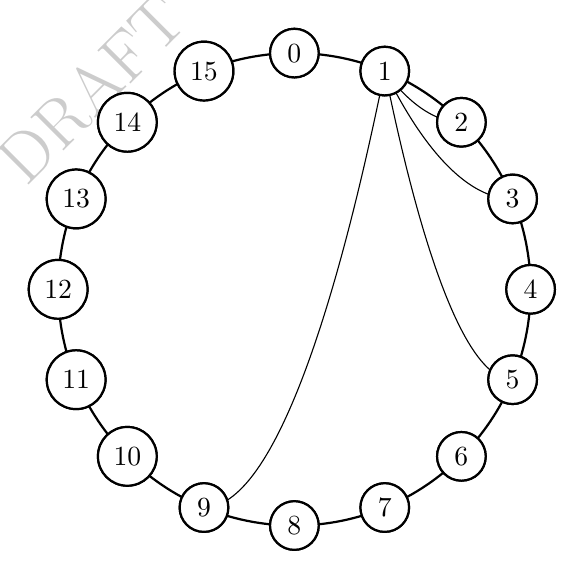
\begin{tikzpicture}[node distance=5cm,auto,>=latex']
    \xdef\N{16}
    \xdef\S{3}
    \xdef\deltadegree{360/\N}
    \draw[thick] (0,0) circle (\S);

    \foreach \i in {0,...,15} {
        % % predecessor
        % \pgfmathsetmacro{\result}{mod(\i-1,\N)}
        % \draw[color=red] (-\i*\deltadegree+90:\S) -- (-1*\result*\deltadegree+90:\S);

        % % successor
        % \pgfmathsetmacro{\result}{mod(\i+1,\N)}
        %     \draw (-\i*\deltadegree+90:\S) -- (-1*\result*\deltadegree+90:\S);

        % fingers
        % \foreach \j in {1,...,4}{
        %     \pgfmathsetmacro{\result}{mod(\i+2^\j,\N)}
        %     \draw (-\i*\deltadegree+90:\S) --- (-1*\result*\deltadegree+90:\S);
        % }
    }
    \foreach \i in {0,...,15}
    \node (\i) [circle,fill=white,draw=black,thick] at (-\i*\deltadegree+90:\S) {\i};
    \draw (1) parabola bend (2) (2);
    \draw (1) parabola bend (3) (3);
    \draw (1) parabola bend (5) (5);
    \draw (1) parabola bend (9) (9);
    \foreach \i in {0,...,15}
    \node (\i) [circle,fill=white,draw=black,thick] at (-\i*\deltadegree+90:\S) {\i};

  \end{tikzpicture}
      \end{center}

      \caption{Chord algorithm, lookup protocol}

    \end{figure}

Algorithm \ref{alg:lookup} locates the successor of a DID or VID. If the local successor sequence can answer the interval query, the transition returns a local owner. Otherwise it returns a remote action naming the next hop and the requested key. The $next = none$ branch is not an ownership claim: after an interval miss it is unreachable in a converged ring, and under partial local state it returns a repair action so the interpreter refreshes successor evidence before retrying. On a converged ring, repeatedly interpreting the remote action resolves to the mathematical successor of the target. The $O(\log N)$ routing expectation depends on sufficiently populated finger tables; correctness still falls back to the successor sequence.

\begin{algorithm}[h]
\caption{DHT Stabilization}
\begin{algorithmic}[1]
\Procedure{Stabilize}{$n, topo$}
\State $actions\gets []$
\State $c\gets topo.pred$
\State $s\gets head(succ[n])$
\If {$c \neq none$ and $c \in (n.did, s)$}
\State $succ[n]\gets insert(succ[n], c)$
\State $actions\gets actions :: FindSuccessor(c)$
\EndIf
\State $succ[n]\gets take(r, merge(succ[n], topo.succ))$
\If{$head(succ[n]) \neq none$}
\State $h\gets head(succ[n])$
\State $actions\gets actions :: Notify(h, n.did)$
\EndIf
\State \Return $Multi(actions)$
\EndProcedure
\end{algorithmic}
\end{algorithm}

The \textbf{stabilization} algorithm is a monotone refinement step over known topology. It accepts a better successor candidate when the current successor reports a predecessor closer to the local node, merges bounded successor-list evidence, and returns actions for follow-up lookup or notification. Finger repair is a separate optimization pass that uses the same biased-distance order. Stabilization improves routing efficiency, storage placement, and hand-off safety, but the formal claim is scoped to convergence toward the Chord safety fixpoint under the modeled assumptions.

\subsection{Virtual DID}

In Rings Network, Virtual DID (VID) serves as a network identifier that resembles a DID in format but does not represent an account-controlled node. A VID is a placement key for a resource, mailbox, service descriptor, subring, or application-specific state object. A VID has no private key and no DID proof; authorization comes from the operation applied to the entry and from signatures or capabilities carried in the entry payload.

For a resource descriptor $x$, a protocol derives a VID with a domain-separated hash, for example $H(\mathtt{rings.resource} \Vert namespace \Vert x)$. Domain separation is required so that a mailbox, a service descriptor, and a storage chunk with the same user-visible name do not collide semantically even if they map into the same 160-bit identifier space.

\textbf{Data storage} is the foundation for advanced data storage operations. When a node stores data, it derives a VID and uses Chord lookup plus configured redundancy to place entries on responsible nodes. Large data is split into chunks; each chunk has its own VID, and the root entry stores a signed manifest containing chunk identifiers, sizes, hashes, encryption metadata, and recovery policy. Storage capacity is an adapter and policy concern, not a fixed global protocol constant.

\textbf{Mailbox} provides asynchronous delivery for DIDs that are offline or unreachable. A mailbox root can be derived as $H(\mathtt{rings.mailbox} \Vert DID \Vert epoch)$, where the epoch limits scanning and storage growth. Senders append encrypted envelopes to the mailbox entry. Each envelope contains the recipient DID, sender session proof or anonymous credential, ciphertext, expiration, replay nonce, and optional postage or ranking evidence. The recipient retrieves mailbox entries by proving control of the DID, decrypts envelopes locally, and acknowledges or garbage-collects messages according to the mailbox policy. This design gives offline delivery without requiring direct interaction, but it does not hide the existence of a mailbox access pattern unless combined with cover traffic or private retrieval.

\textbf{Hidden services} are service descriptors stored under VIDs rather than ordinary DNS names. A descriptor contains a service namespace, rendezvous policy, relay or introduction points, capability requirements, public keys, expiration, and ranking/admission constraints. Clients look up the descriptor, verify its signature, choose an introduction path, and establish an encrypted application session through the overlay. Service pseudonymity and server-location privacy are limited to the protections provided by the descriptor, relay-path selection, and traffic-analysis defenses.

\textbf{Sub Ring} is a scoped overlay whose membership and routing state are anchored by a VID. The subring name or policy derives the subring VID, while members join by submitting signed membership operations. The DHT-persisted state stores the membership log or a compact joined state; participants keep local finger tables using the subring's fixed point and membership set. Convergence requires that join operations are idempotent and mergeable, that conflicting membership updates have deterministic resolution, and that stale members expire or are removed by signed policy operations.

\section{Traffic}

In Rings Network, the abstraction of traffic is divided into two approaches: Hop-by-Hop and End-to-End. Hop-by-Hop refers to a communication architecture where data is transmitted from one device to another through multiple intermediate systems in between. On the other hand, End-to-End (E2E) refers to a communication architecture where data is transmitted directly from the sender's device to the recipient's device without passing through any intermediate systems.


\subsection{Hop by Hop}

In Rings Network, a structured peer-to-peer network, accounts prove DID ownership with account signature algorithms, then delegate a time-bounded session keypair. Each hop carries signed message payloads, routing metadata, and typed messages. The overlay infers a next hop from the local DHT when a direct transport connection to the final destination is not available.

The message relay and chunking layers borrow concepts from MSRP-style message splitting \cite{RFC4975}, but Rings defines its own relay semantics instead of claiming MSRP compliance. A Rings relay frame contains the path state needed by the overlay, a destination DID or VID, a namespace, a signed session proof, and either an application payload or a report. Reports acknowledge delivery, failure, forwarding refusal, or storage placement, giving applications enough information to retry or choose a different path.

\subsection{End to End}

Rings Network places significant emphasis on End-to-End Encryption as a means to ensure privacy and security. The target E2E protocol uses public keys that are proven to match the signed sender or recipient DID. RSA is not part of the Rings target unless a later design explicitly reintroduces it; the privacy layer uses elliptic-curve encryption, signed envelopes, and cryptographic carriers that can support private computation.

Given an elliptic-curve cyclic group $\mathbb{G}$ of order $q$ with generator $g$, a private key $x \in \mathbb{Z}_q$, and public key $h = g^x$, Algorithm \ref{alg:elgamal} summarizes the ElGamal operation:

\begin{algorithm}[h]
\caption{ElGamal Encryption and Decryption}
\label{alg:elgamal}
\begin{algorithmic}[1]
\State \textbf{Input:} Message $m$, private key $x \in \mathbb{Z}_q$, public key $h = g^x$, generator $g$
\State \textbf{Output:} Encrypted message $(c_1, c_2)$
\Procedure{Encryption}{}
\State Choose a random integer $k \in \mathbb{Z}_q$
\State Compute $c_1 = g^k$
\State Compute $c_2 = m\cdot h^k$
\State \Return $(c_1, c_2)$
\EndProcedure
\Procedure{Decryption}{}
\State Compute $m = c_2\cdot(c_1)^{-x}$
\State \Return $m$
\EndProcedure
\end{algorithmic}
\end{algorithm}

An encrypted stream divides byte payloads into ordered frames. Each frame carries a stream identifier, sender public key, monotonic sequence, final marker, and ciphertext blocks. The frame is then carried in a signed message envelope, which supplies sender authentication, public-key ownership, frame integrity, and truncation detection.

Secret sharing is a separate privacy-layer primitive. The secret is first encoded over an appropriate finite field, for example with a threshold polynomial. Shares are then encrypted to participant keys and placed on the overlay by VID. The Chord identifier space decides where shares live; it is not the field in which the threshold scheme is computed. Recovery requires at least the threshold number of valid shares plus the corresponding decryption authority.

 \subsection{Chunking}

 When the size of a message exceeds the negotiated transport message size, Rings splits the payload into ordered chunks and reassembles the original payload once all chunks arrive. The safe baseline is whole-message buffering with bounded reassembly: the receiver accepts out-of-order chunks, ignores duplicate positions, drops partial messages by TTL, and enforces per-message and total memory limits. Streaming mode is outside the baseline until interruption, partial-delivery, and backpressure semantics are specified explicitly.

 \begin{algorithm}[h]
\caption{End-to-End Chunking Algorithm}
\label{alg:e2e_chunking}
\begin{algorithmic}[1]
\Procedure{E2E Chunking}{}
\State Input: data, chunk size
\State Output: chunks
\State chunks $\gets$ []
\State total-chunks $\gets$ ceil(len(data)/chunk-size)
\For{i in range(total-chunks)}
\State chunk $\gets$ data[i*chunk-size : (i+1)*chunk-size]
\State append chunk to chunks
\EndFor
\State \Return chunks
\EndProcedure
\end{algorithmic}
\end{algorithm}

Algorithm \ref{alg:e2e_chunking} shows the sender-side shape of whole-message chunking. A robust receiver also validates timestamps, per-chunk size, total chunk count, total buffered cost, and completed-message tombstones.

\section{Sequencer and Ranking}

A sequencer in a distributed system is a component responsible for determining the order in which messages are delivered or transactions are executed. Rings does not embed a global consensus system into the base overlay; doing so would turn the network into a blockchain rather than a sovereign peer-to-peer substrate. Instead, Rings uses local protocol ordering where possible and sidecar witnesses where a stronger ordering proof is required.

\subsection{Sidecar Sequencer}

The Sidecar Sequencer is a witness protocol, not a mandatory base-layer consensus engine. A message that requires ordering carries a witness reference such as a block hash, timestamped commitment, signed log root, or application-specific ordering certificate. The verifier checks three facts:

\begin{itemize}[itemsep=2pt,topsep=0pt,parsep=0pt]
\item the witness existed before or after a claimed bound;
\item the message commitment is bound to that witness;
\item the application accepts the witness source and its finality rule.
\end{itemize}

Sidecar sequencing therefore gives a partial order unless all compared messages use the same finality domain or the application defines a cross-domain comparison rule. If Message A is witnessed by Bitcoin and Message B by Solana, Rings cannot infer a universal total order from those witnesses alone. The application either accepts a partial order, chooses a canonical witness domain, or defines a deterministic tie-breaker.

\subsection{Byzantine Fault Boundary}

Rings does not solve Byzantine fault tolerance for every application at the overlay layer. It delegates ordering finality to the selected sidecar witness and verifies that the witness is correctly attached to a Rings message. This keeps the overlay small while allowing applications to select different security assumptions: a blockchain, a threshold signature committee, a transparency log, or a local Lamport-style clock for weaker ordering needs.

\subsection{Ranking Protocol}

The target Ranking Protocol turns peer quality into a signed, challengeable, and rate-limited signal. A ranking event contains:

\begin{itemize}[itemsep=2pt,topsep=0pt,parsep=0pt]
\item the subject DID and rater DID;
\item the measured behavior, such as connection success, delivery success, storage availability, latency bucket, or protocol violation;
\item evidence, such as signed reports, failed challenge transcripts, or availability probes;
\item an epoch, expiration, and anti-replay nonce;
\item the rater's stake, credential, or trust weight.
\end{itemize}

Scores are aggregated by epoch with robust statistics such as median or trimmed mean so that outliers do not dominate. The ranking result is not a moral identity score; it is an operational routing and admission signal. A node may use ranking to choose relay paths, reject storage writes, select mailbox replicas, throttle spam, or require stronger payment/proof from low-quality peers.

Sybil resistance requires more than peer voting. The protocol combines admission cost, proof-of-work or stake, social or issuer credentials, freeze periods for new rank claims, and challenge/slashing rules for false evidence. A low-ranked node can recover by producing fresh good evidence, while a malicious high-ranked node loses score when challenged with signed failure evidence.

\section{Performance}

The performance discussion separates latency from reliability and treats Chord measurements as reference data rather than Rings deployment evidence.

\subsection{Latency}
For Rings Network, latency mainly comes from transport establishment, lookup/routing through the Chord overlay, relay path length, sidecar witness verification, and application protocol work such as encryption or proof verification. The Chord reference data below is useful for reasoning about expected lookup behavior, but it is not a substitute for Rings-owned measurements under browser, native, NAT, relay, and churn conditions.

\begin{table}[htbp]
\begin{tabular}{l|l|l}
\cline{1-3}
  \shortstack{Fraction of \\failed nodes} & \shortstack{Mean \\routing hops} &\shortstack{Mean num. of \\lookup timeouts}   \\ \cline{1-3}
0                        & 3.84             & 0.0                     \\ \cline{1-3}
0.1                      & 4.03             & 0.60                    \\ \cline{1-3}
0.2                      & 4.22             & 1.17                    \\ \cline{1-3}
\end{tabular}
\caption{Latency on failed node rate of Chord \cite{Chord}}
\end{table}

\begin{figure*}[htbp]
  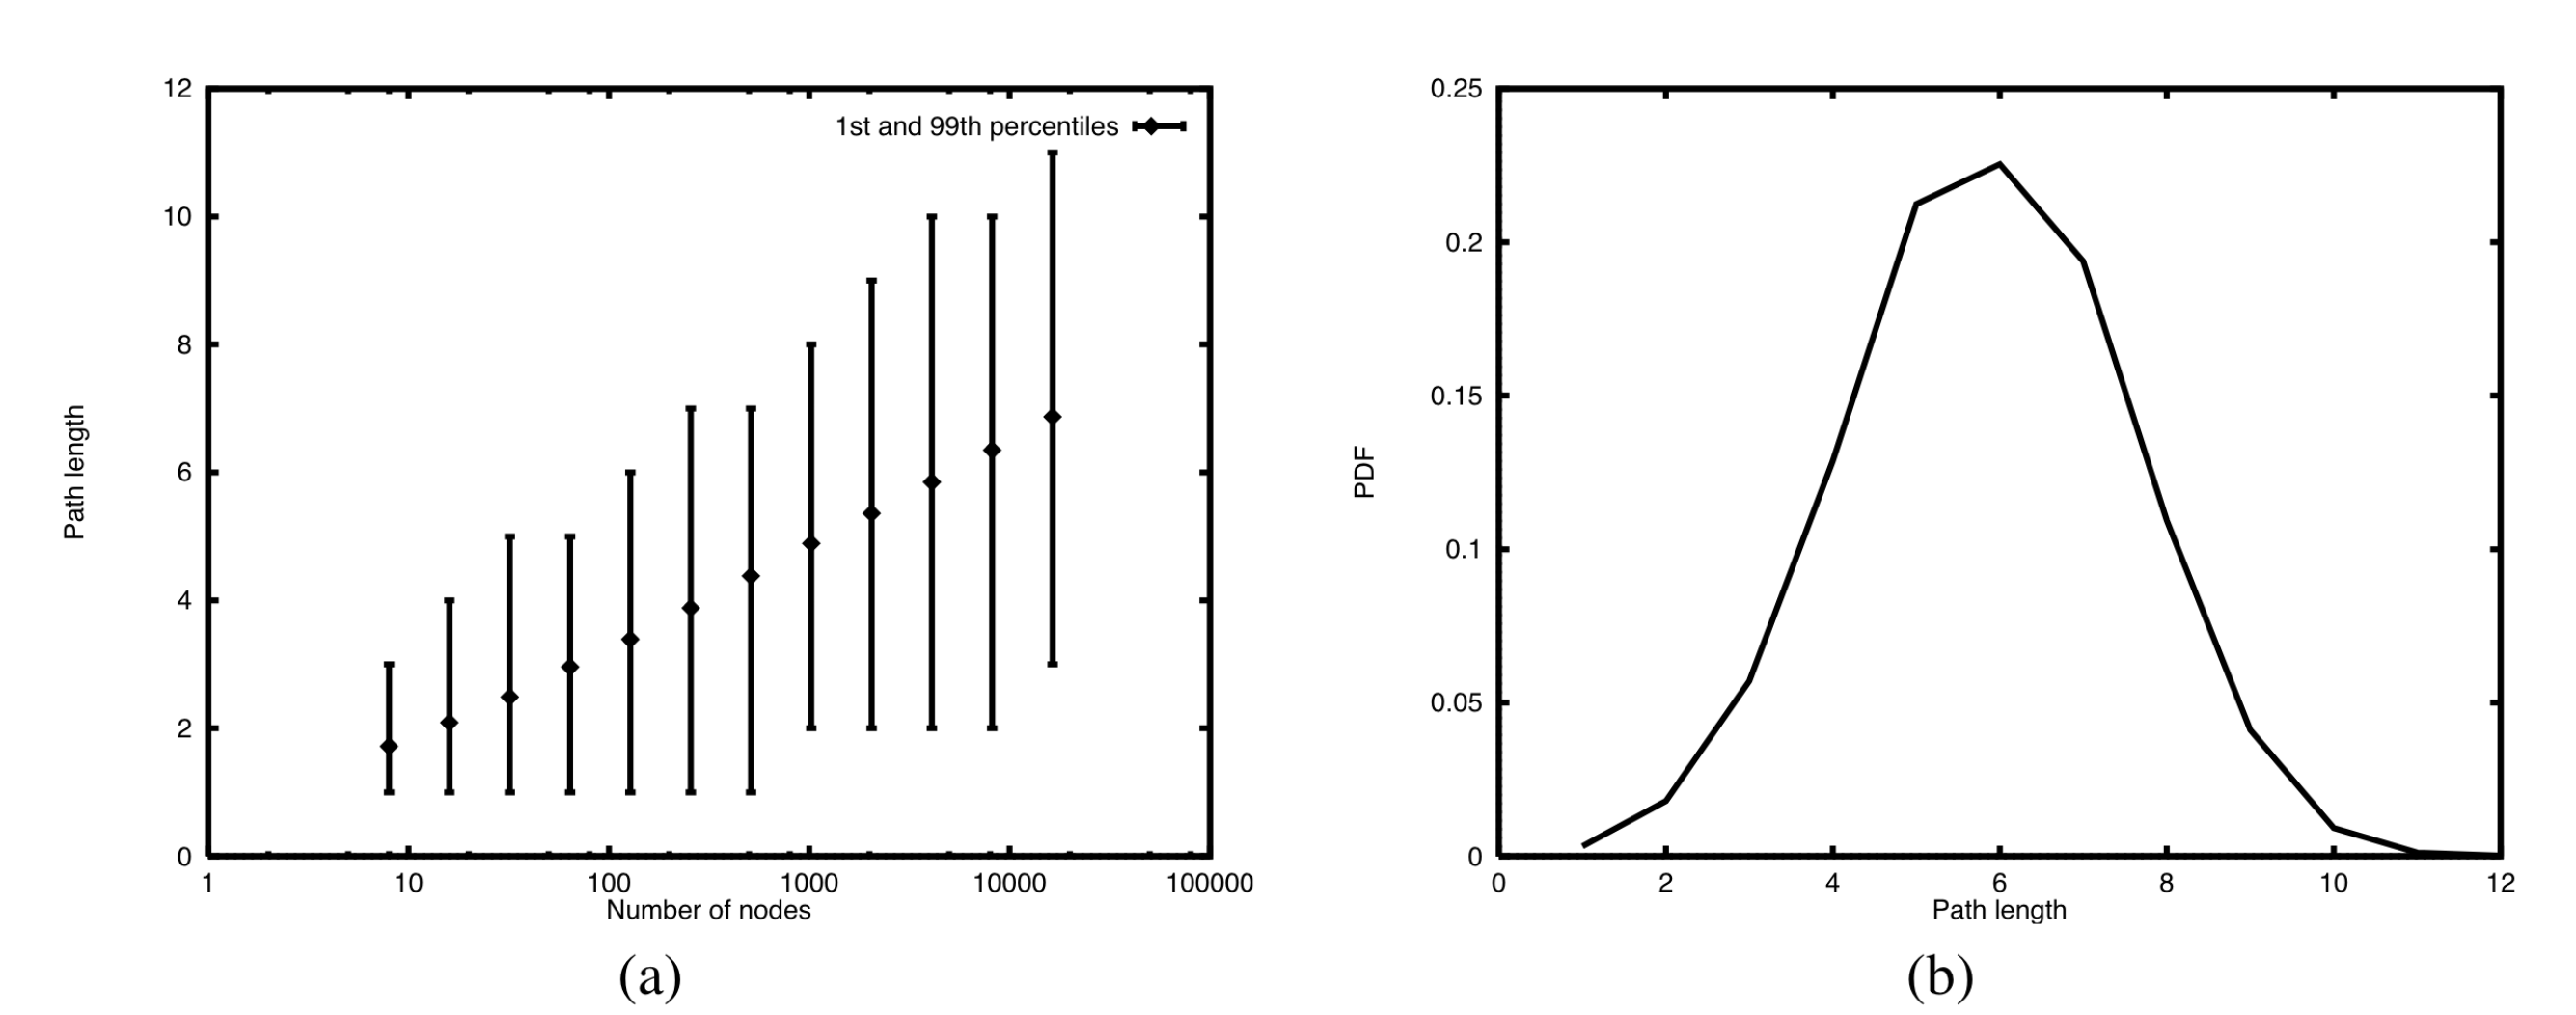
\includegraphics[width=\linewidth]{imgs/rings/path.png}
  \caption{Chord lookup path \cite{Chord}}
  \label{path}
\end{figure*}

According to the cited Chord simulation results, when the number of nodes increases from 10 to 100K, the path length only increases by about 3 times. The left side of Figure \ref{path} shows this scenario, and the right side is the PDF (probability density function) of the path length. Rings treats this as a Chord reference expectation until measured under its own transport and application workloads.
\subsection{Reliability}

Rings Network allows browser nodes to participate directly in the overlay, which increases expected join and leave rates. Hence, the network's performance with frequent node churn is crucial for evaluation. Browser nodes may have equal protocol authority without identical persistence, socket, or background-execution capabilities.

\begin{table}[htpb]

  \begin{tabular}{l|l|l|l}
\cline{1-4}
  \shortstack{join/leave rate \\ (per sec./stab. \\ period)}
  & \shortstack{Mean \\routing\\ hops}
  &\shortstack{Mean \\num. of \\lookup \\timeouts}
  &\shortstack{Lookup \\ failures \\ per 10k} \\ \cline{1-4}
0.05/1.5                        & 3.90             & 0.5              &    0   \\ \cline{1-4}
0.10/2                      & 3.83             & 0.11             &    0   \\ \cline{1-4}
  0.15/4.5                      & 3.84             & 0.16             &    2   \\ \cline{1-4}

  0.20/6                      & 3.81             & 0.23             &    5   \\ \cline{1-4}
0.25/7.5                      & 3.83             & 0.30             &    6   \\ \cline{1-4}
  0.30/9                      & 3.91             & 0.34             &    8   \\ \cline{1-4}
  0.35/10.5                      & 3.94             & 0.42             &    16   \\ \cline{1-4}
0.40/12                      & 4.06             & 0.46             &    15   \\ \cline{1-4}

\end{tabular}
\caption{Failure rate of Chord \cite{Chord}}
\label{failure}
\end{table}

Table \ref{failure} shows Chord reference simulation results under increasing join/leave rates. Rings treats these numbers as theoretical guidance; concrete availability claims require independent measurements for the full protocol stack.


\section{Security}
As a decentralized platform, Rings Network has security exposure at the identity, routing, storage, relay, and application layers. The target model scopes the following attacks and mitigations:
\begin{itemize}[itemsep=2pt,topsep=0pt,parsep=0pt]
\item Sybil Attack: A Sybil attack represents a malicious attempt to undermine the trust and control of a network by creating multiple fake identities. The target Ranking protocol mitigates this through admission cost, signed evidence, freeze periods, challengeable claims, and local/global routing signals. Ranking reduces Sybil impact; it does not eliminate Sybil attacks without an economic or credential cost model.

\item Replay Attack:
  A replay attack constitutes a malicious attempt to disrupt a network by intercepting and retransmitting a legitimate network transmission. Rings uses digital signatures, cryptographic hashes, timestamps, TTLs, nonces, session expiration, and application-level sequence numbers to limit replay. A Sidecar Sequencer can strengthen replay prevention for critical ordered messages, but only within the finality and comparison rules of the selected witness.

\item Man-in-the-Middle Attack:
  A man-in-the-middle (MITM) attack represents a malicious attempt to intercept and potentially modify or eavesdrop on communication between two parties. Rings mitigates MITM attacks by validating signatures, binding public keys to DIDs, signing message envelopes, and encrypting end-to-end payloads. Metadata and traffic-analysis risks remain separate concerns.

\item Denial of Service Attack
A denial-of-service (DoS) attack is a type of cyberattack where an attacker sends a large volume of requests to a network to overwhelm it and disrupt its normal functioning. Rings mitigates DoS through rate limits, bounded chunk reassembly, storage admission policy, ranking, relay quotas, and application-specific costs. These mechanisms bound damage rather than guaranteeing universal availability.
\end{itemize}

\section{Conclusion}
This paper presents Rings Network as a target decentralized, peer-to-peer architecture for the digital era of sovereignty. In the ideal model, Rings combines WebRTC, WebAssembly, DID proofs, Chord-derived lookup, signed sessions, encrypted messages, and virtual DIDs to support secure communication, data placement, and service discovery. The remaining engineering task is to validate these protocol claims with implementation-specific measurements, failure models, and extension-runtime constraints.

\bibliographystyle{unsrt}
\bibliography{./cites}
\end{document}
